\section{Design}
FlashEigen is an external-memory eigensolver optimized for any fast I/O devices
such as a large SSD array to compute eigenvalues of sparse graphs. It takes
advantage of the flexible programming interface of the Anasazi framework and
focuses on optimizing sparse matrix sparse matrix multiplication and dense
matrix operations on SSDs.

\subsection{Eigensolver algorithm}

%\begin{figure}
%\centering
%\includegraphics[scale=0.35]{./SpMM.pdf}
%\vspace{-5pt}
%\caption{}
%\vspace{-5pt}
%\label{SpMM}
%\end{figure}

\begin{algorithm}
	\begin{algorithmic}[1]
		\For{i = 0, 1, ..., until convergence}
		\State (1) Update the subspace $S \in \mathbb{R}^{n \times m}$,
		\State (2) Solve the projected eigenproblem $S^TASy = S^TSy\theta$.
		\State (3) Compute the residual: $r = Kx - x\theta$, where
		\State\hspace{\algorithmicindent} $x = Sy$ (Ritz vector), $\theta = \rho(x)$ (Ritz value).
		\State (4) Test the convergence of a Ritz pair $(x, \rho(x))$.
		\EndFor
	\end{algorithmic}
	\caption{Pseudo code of a generic eigenvalue algorithm that compute eigenvalues
	of a square matrix $A$ with $n$ rows and columns.}
	\label{eigencode}
\end{algorithm}

The state-of-art eigenvalue algorithms compute eigenvalues with iterative
methods. Figure \ref{eigencode} shows the steps in an iteration.
Step (1) constructs a vector subspace $S \in \mathbb{R}^{n \times m}$, where
$n$ is the number of rows or columns of a sparse matrix and $m$ is the number
of vectors in the subspace. When computing eigenvalues of a sparse graph,
two key operations in this step are sparse matrix multiplication to construct
the subspace and reorthogonalization to fix float-point rounding errors.
A block extenion of an eigensolver updates multiple vectors in the subspace
in a single step, which leads to sparse matrix dense matrix multiplication.

\subsection{The architecture of FlashEigen}

We build FlashEigen on top of SAFS, a user-space filesystem, to fully utilize
the I/O throughput of a large SSD array. The architecture of FlashEigen is shown
in Figure \ref{arch}. FlashEigen stores data of sparse matrices and dense matrices
in SAFS and implements matrix operations required by the Anasazi eigensolvers.
As such, the Anasazi eigensolvers can access data from SSDs.

\begin{figure}
\centering
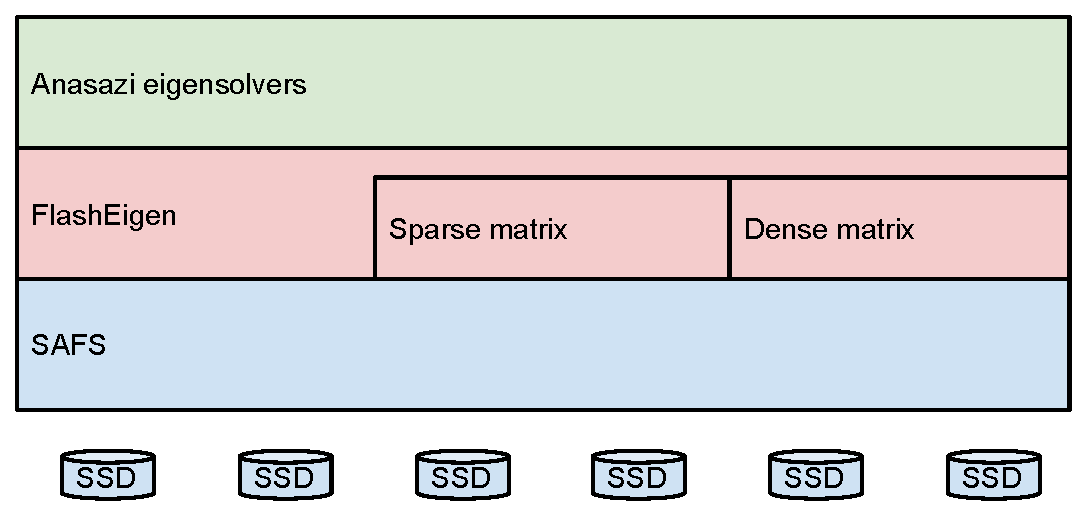
\includegraphics[scale=0.4]{./architecture.pdf}
\vspace{-5pt}
\caption{The architecture of FlashEigen.}
\vspace{-5pt}
\label{arch}
\end{figure}

\subsection{SAFS}

SAFS \cite{safs} is a user-space filesystem for a high-speed SSD array in
a NUMA machine. It is implemented as a library and runs in the address space
of its application. It is deployed on top of the Linux native filesystem.
SAFS was originally designed for optimizing small I/O accesses. However,
sparse matrix dense matrix multiplication and dense matrix operations
generates much fewer but much larger I/O. Therefore, we provide additional
optimizations to maximize sequential I/O throughput from a large SSD array.

The original SAFS has a dedicated I/O thread for each SSD and application threads
have to send I/O requests to one of the I/O threads when accessing data from SSDs.
As such, an I/O thread accesses an SSD exclusively. This strategy avoids lock
contention in the Linux kernel, but potentially increases the number of thread
context switches for I/O access. The cost of a context switch is amortized by
having applications to issue many I/O requests.

The latency of a thread context switch becomes noticeable on a high-speed SSD
array under a sequential I/O workload and it becomes critical to avoid thread
context switch to gain I/O performance. Under such a workload, each I/O thread
gets much fewer parallel I/O requests from an application and each I/O completion
may suffer from the latency of a context switch.
Therefore, instead of having an I/O thread for each SSD \cite{safs}, we
use only a single I/O thread for each NUMA node, which is responsible for
all of the SSDs connected to the NUMA node. As such, an I/O thread processes
many more I/O requests to amortize the latency of a context switch.
Similarly, if the computation in application threads did not saturate CPU,
SAFS would put the application threads into sleep while they were waiting
for I/O. This results in many thread context switches and, thus, both CPU and
SSDs were under utilization. To saturate I/O, an application thread continues
issuing asynchronous I/O. However, instead of getting notified of I/O completion,
application threads poll for I/O to avoid thread context switches when they
complete all computation available to it.

To better support access to many relatively small files simultaneously,
SAFS stripes data in a file across SSDs with a different
striping order for each file to store data evenly across SSDs and improve
I/O utialization. Due to the sequential I/O workload from FlashEigen,
we stripe data across SSDs with a large block size, in the order of multiple
megabytes, to increase I/O throughput and potentially reduce write amplification
on SSDs \cite{}. Such a large block size may cause storage skew on a large SSD
array if every file stripes data in the same order.
The same striping order may also cause more I/O accesses to hit some of the SSDs
and saturate them while other SSDs are under utilization. Therefore, whenever
a new file is created, SAFS generates a random striping order for the file to
evenly distribute I/O among SSDs. SAFS stores the striping order with the file
for future data retrieval from the file.

\dz{fair I/O scheduling}

\dz{use a large I/O blocks in the kernel}

\subsection{Sparse matrix multiplication} \label{spmm}
Sparse matrix multiplication is a computationally expensive
operation in an eigensolver due to random memory access. Sparse matrix vector
multiplication (SpMV) is usually limited by the random memory performance of
DRAM. Sparse matrix dense matrix multiplication (SpMM) increases data locality
and improve overall performance of an eigensolver. Therefore, a block extension
of an eigensolver is preferred.

To handle a sparse graph with billions of vertices, we perform sparse matrix
multiplication in semi-external memory (SEM),
i.e., the input and output vectors or dense matrices in memory and the sparse
matrix on SSDs. This strategy enables nearly in-memory performance while achieving
the scalability in proportion to the ratio of edges to vertices in a graph.

\subsubsection{The sparse matrix format}
The state-of-art numeric libraries store a sparse matrix in compressed row storage
(CSR) or compressed column storage (CSC) format. However, these formats incur
many CPU cache misses in sparse matrix multiplication on many real-world graphs
due to their nearly random vertex connection. They also require a relatively
large storage size. For a graph with billions of edges, we have to use eight
bytes to store the row and column indices. For semi-external memory sparse
matrix multiplication, a large matrix format may cause SSDs to be the bottleneck.
Therefore, we need to use an alternative format for sparse matrices to increase
CPU cache hits and reduce the amount of data read from SSDs.

\begin{figure}
\centering
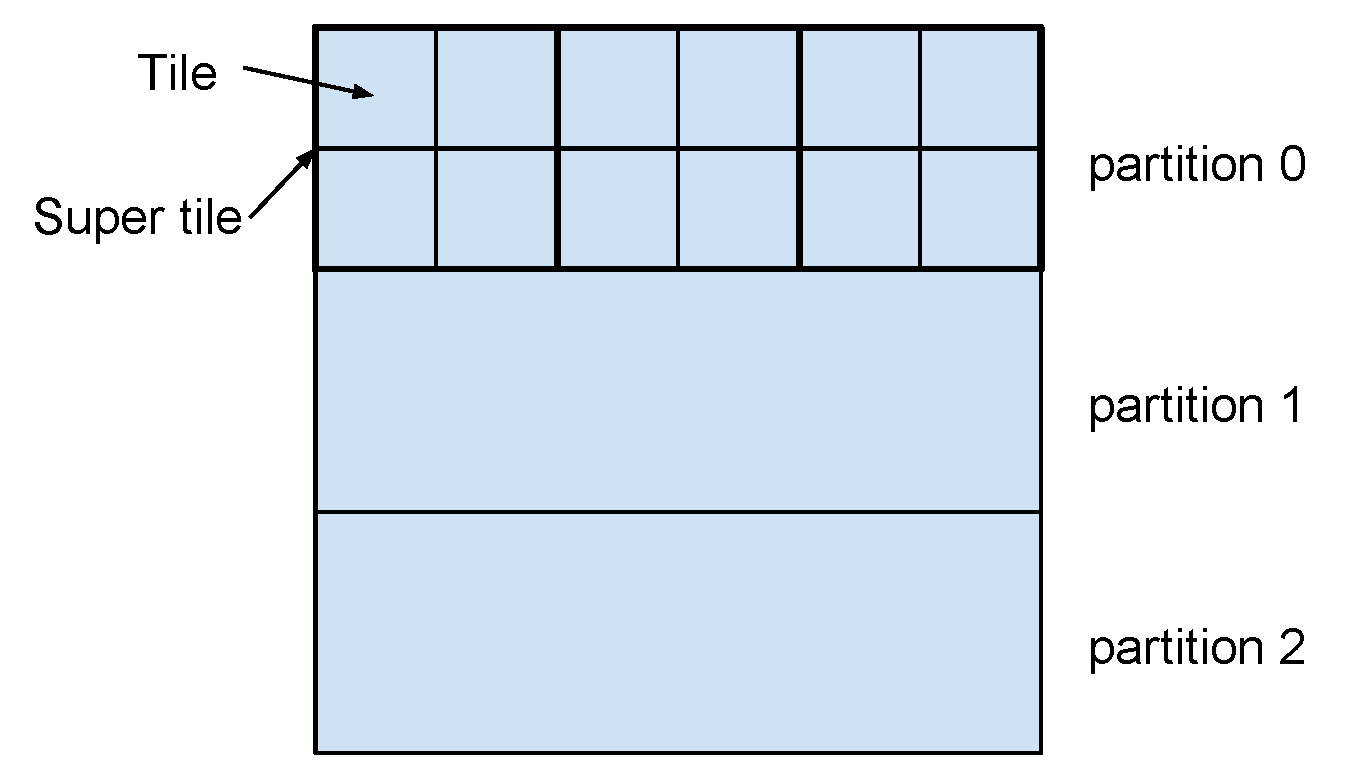
\includegraphics[scale=0.3]{./sparse_mat.pdf}
\vspace{-5pt}
\caption{}
\vspace{-5pt}
\label{sparse_mat}
\end{figure}

To increase CPU cache hits, we deploy cache blocking \cite{Im04} and store
non-zero entries in a sparse matrix in tiles (Figure \ref{sparse_mat}).
When a tile is small, the rows of the input and output dense matrices
involved in the multiplication with the tile are always kept in the CPU cache
during the multiplication. The optimal tile size should fill the CPU cache
with the rows of the dense matrices involved in the multiplication with
the tile and is affected by the number of columns of the dense matrices.
The number of columns of these dense matrices are chosen by users. Instead
of generating a sparse matrix with
different tile sizes optimized for different numbers of columns in the dense
matrices, we use a relatively small tile size and rely on the runtime system
to optimize for different numbers of columns (in section \ref{sec:exec}).
In the semi-external memory mode, we expect that the dense matrices do not
have more than eight columns in sparse matrix multiplication. By default, we
use the tile size of $16K \times 16K$ to the matrix storage size and
the adaptibility to different numbers of columns.

\begin{figure}
\centering
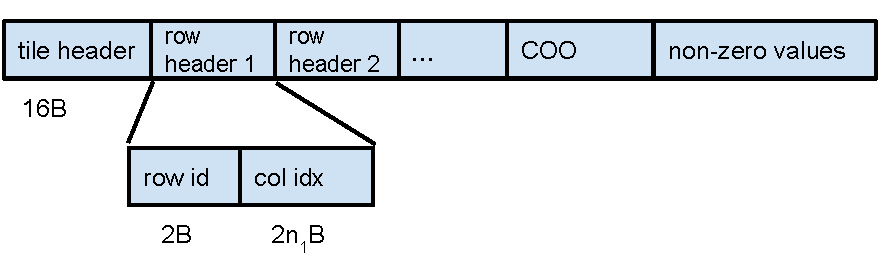
\includegraphics[scale=0.5]{./tile_format.pdf}
\vspace{-5pt}
\caption{The storage format of a tile in a sparse matrix.}
\vspace{-5pt}
\label{tile_format}
\end{figure}

To reduce the overall storage size of a sparse matrix, we use a compact format
to store non-zero entries in a tile. In very sparse matrices such as
many real-world graphs, many rows in a tile do not have any non-zero entries.
The CSR (CSC) format requires an entry for each row (column) in the row
(column) index. Therefore, the CSR or CSC format waste space when storing elements
in a tile. Instead, we only keeps data for rows with non-zero entries in a tile
shown in Figure \ref{tile_format}. For rows with more than one non-zero entries,
we use a variant of the CSR format, which maintains a row header for each row.
A row header has an identifier to indicate the row number, followed by column
indices. We refer to this format as SCSR (Super Compressed Row Storage).
The most significant bit of the identifier is always set to 1, while the most
significant bit of a column index entry is always set to 0. As such, we can easily
distinguish a row identifier from a column index entry and determine the end
of a row. Thanks to the small size of a tile, we use two bytes to store a row
number and a column index entry to reduce the storage size. Since the most
significant bit is used to indicate the beginning of a row, the maximum tile size
is $32K \times 32K$.

For many real-world graphs, many rows in a tile have only one non-zero entries,
thanks to their nearly random vertex connection. Storing these single-entry
rows in separate rows results in many conditional jump CPU instructions in
sparse matrix multiplication.
In contrast, the coordinate format (COO) is more suitable for storing these
single-entry rows. It does not increase the storage size but significantly
reduces the number of conditional jump instructions when we iterate
them. As a result, we hybrid SCSR and COO to store non-zero entries in a tile
with COO stored behind the row headers of SCSR. All non-zero entries are
stored together at the end of a tile.

We organize tiles in a sparse matrix in tile rows and maintain a matrix index
for them. Each entry of the index stores the location of a tile row on SSDs
to facilitate random access
to tile rows. This is useful for parallelizing sparse matrix multiplication.
Because a tile contains thousands of rows, the matrix index requires a very
small storage size even for a billion-node graph. We keep the entire index
in memory during sparse matrix multiplication.

\subsubsection{The dense matrix format for SpMM} \label{numa_mat}
The dense matrix in sparse matrix multiplication is a tall-and-skinny matrix
with millions or even billions of rows but only several columns. For sparse
matrix multiplication, we organize elements of the dense matrix in row-major
order to increase data locallity, as shown in Figure \ref{dense_mat} (a).

For a non-uniform memory architecture (NUMA), we partition the input dense matrix
horizontally and store partitions evenly across NUMA nodes to fully utilize
the bandwidth of memory and inter-processor links in sparse matrix
multiplication. The NUMA architecture is commonly used in today's multi-processor
servers, where each processor connects to its own memory banks. It is essential
to fully utilize the bandwidth of memory and inter-processor links to achieve
performance. As shown in Figure \ref{dense_mat} (a), we assign multiple
contiguous rows to a partition and assign multiple partitions to the same
NUMA node. A partition always has $2^i$ rows for efficiently locating a row
with bit operations. The partition size is also multiple of the tile size of
a sparse matrix so that multiplication on a tile only needs to access rows
from a single partition.

\begin{figure}
\centering
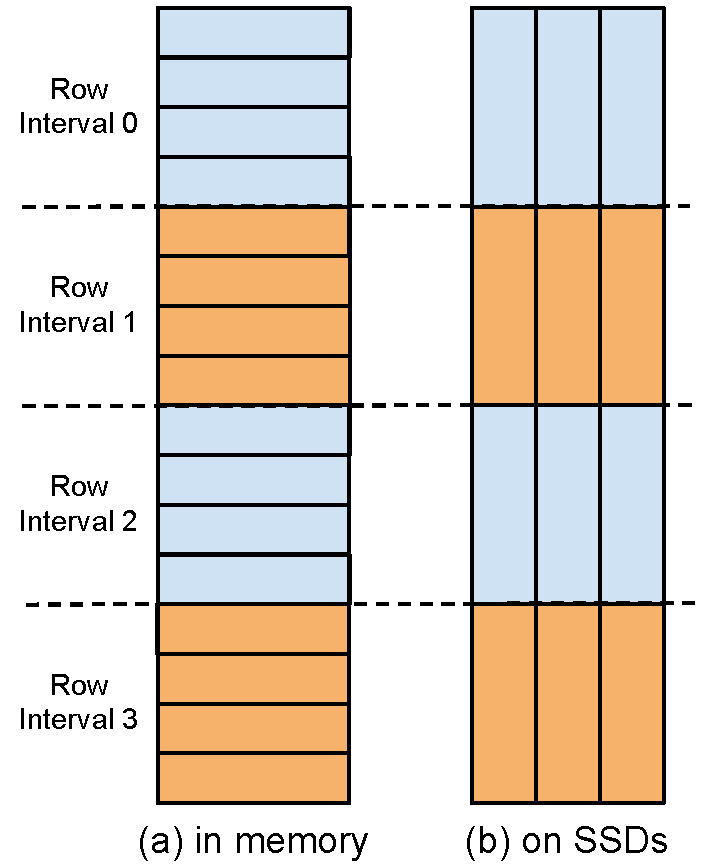
\includegraphics[scale=0.4]{./dense_matrix.pdf}
\vspace{-5pt}
\caption{The data layout of tall-and-skinny dense matrices. A tall-and-skinny
dense matrix is partitioned horizontally into many row intervals.
(a) For an in-memory matrix, row intervals are stored across NUMA nodes and
elements are stored in row-major order; (b) for an SSD-based matrix, elements
inside a partition are stored in column-major order.}
\vspace{-5pt}
\label{dense_mat}
\end{figure}

\subsubsection{Execution of sparse matrix multiplication} \label{sec:exec}
We perform sparse matrix dense matrix in semi-external memory.
We optimize sparse matrix dense matrix multiplication at runtime for different
numbers of columns in the dense matrices.

We partition a sparse matrix horizontally for parallelization and assign multiple
contiguous tile rows to the same partition (Figure \ref{sparse_mat}).
The number of tile rows assigned to a partition is determined at runtime by
the number of columns in the input dense matrix.
\dz{Can we just give a fixed number of tile rows to a partition and use
the hilbert curve to process tiles?}
A thread reads a partition of the sparse matrix
asynchronously from SSDs. Once a partition is ready in memory, the worker
thread multiplies the partition with the input dense matrix and allocates
a buffer in the local memory to store the result. To reduce memory consumption,
we write the portion of the output dense matrix to SSDs immediately whenever
it is generated. \dz{Implement this.}

To better utilize CPU cache, we process tiles of a partition in
\textit{super tile}s (Figure \ref{sparse_mat}). The tile size of a sparse
matrix is specified when the sparse matrix image is created and is relatively
small to handle different numbers of columns in the dense matrices.
A \textit{super tile} is composed of tiles from multiple tile rows and its
size is determined at runtime by three factors: the number of columns
in the dense matrices, the CPU cache size and the number of threads that
share the CPU cache. An optimal size for a \textit{super tile} fills
the CPU cache with the rows from the dense matrices involved in
the computation with the \textit{super tile}.
\dz{Should I give an example here?}

Load balancing also plays a key role in sparse matrix multiplication on
many real-world graphs due to their power-law distribution in vertex degree.
In FlashEigen, a worker thread first processes partitions with more non-zero
entries, originally assigned to the thread. When a worker thread finishes
all of its own partitions, it steals partitions that have not been processed
from other worker threads.

In spite of nearly random distribution of non-zero entries in a sparse matrix,
there exists regularity that allows vectorization to improve performance
in sparse matrix dense matrix multiplication. For each non-zero entry, we
need to multiply it with the corresponding row from the input dense matrix
and add the result to the corresponding row in the output dense matrix.
These operations can be accomplished by the vector CPU instructions such as
AVX \cite{avx}. The current implementation relies on GCC's auto-vectorization
to translate the C code to the vector CPU instructions by predefining the matrix
width in the code.

\subsection{Dense matrix operations}
The vector subspace required by an eigensolver is massive when the eigensolver
computes eigenvalues of a billion-node graph or computes many eigenvalues
of a multi-million-node graph. The number of vectors in the subspace
increases with the number of required eigenvalues. Furthermore, a larger
number of vectors in the subspace improves the convergence rate of an eigensolver. 
It is often that an eigensolver needs multiple terabytes to store the vectors
in the subspace for eigenvalue problems at such a scale. Therefore, FlashEigen
stores vectors on SSDs.

FlashEigen stores multiple vectors of the subspace in a dense matrix physically.
One reason is that the Anasazi eigensolvers update multiple vectors of the subspace
in an iteration due to the block extension of the eigenvalue algorithms.
The number of vectors stored in a matrix is determined by the block size of
a block eigensolver.
This design also helps garbage collection in lazy evaluation (section \ref{sec:lazy_eval}).
As such, the subspace is composed of tall-and-skinny dense matrices.
However, the eigensolvers still need to access individual vectors,
so we organize the elements in the dense matrices in column-major order. 

\begin{table}
	\begin{center}
		\small
		\begin{tabular}{|c|c|c|c|c|}
			\hline
			& operation & customized output \\
			\hline
			op1 & $CC \leftarrow \alpha \times AA \times B + \beta \times CC$ & yes \\
			\hline
			op2 & $BB \leftarrow AA \times diag(vec)$ & yes \\
			\hline
			op3 & $A \leftarrow \alpha \times t(AA) \times BB$ & no \\
			\hline
			op4 & $CC \leftarrow \alpha \times AA + \beta \times BB$ & yes \\
			\hline
			op5 & $BB \leftarrow \alpha \times AA$ & yes \\
			\hline
			op6 & $vec \leftarrow norm\_col(AA)$ & no \\
			\hline
			op7 & $BB \leftarrow AA[,idxs]$ & yes \\
			\hline
			op8 & $AA[,idxs] \leftarrow BB$ & yes \\
			\hline
			op9 & $AA \leftarrow conv\_layout(BB)$ & yes \\
			\hline
		\end{tabular}
		\normalsize
	\end{center}
	\caption{The dense matrix operations required by the Anasazi eigensolvers.
		$XX$ represents a tall dense matrix, $X$ represents a small dense matrix,
	$\alpha$ and $\beta$ represents scalar variables.}
	\label{anasazi_ops}
\end{table}

The Anasazi eigensolvers allow users to implement
the tall-and-skinny matrices and their operations. Such flexibility allows us to
store dense matrices on SSDs or even physically not store a dense matrix.

FlashEigen require a set of dense matrix operations shown in Table
\ref{anasazi_ops}. $op1-8$ are the operations required by the original Anasazi
eigensolvers. The most computationally expensive operations are the two
matrix multiplication operations: $op1$ and $op3$, mainly used for
reorthogonalization to fix float-point rounding errors.
$op7$ and $op8$ access individual columns of a dense matrix.
Therefore, we store the dense matrices in column major by default.
However, the sparse matrix dense matrix multiplication described in section
\ref{spmm} requires a row-major dense matrix to increase data locality.
Thus, FlashEigen adds another operation $op9$ to convert data layout
in dense matrices, which converts a column-major matrix to a row-major
matrix when it is passed to the SpMM operation.

It is challenging to achieve the performance of external-memory dense matrix
operations comparable to their in-memory counterparts. Unlike sparse matrix
multiplication, these dense matrix operations are less \dz{computationally
expensive}. Even though SSDs are fast, their sequential I/O performance is
still an order of magnitude slower than RAM. Therefore, dense matrix operations
on SSDs are significantly slower than the ones in RAM (Figure \ref{perf:mat_ops}).
Furthermore, SSDs wears out after a certain amount of write \cite{}.
Even enterprise SSDs \cite{} only allows a small number of DWPD
(diskful writes per day). Therefore, FlashEigen optimizes dense matrix operations
with the goals of maximizing I/O throughput from SSDs and minimizing the amount
of data read and written to SSDs.

%\begin{figure}
%	\begin{center}
%		\footnotesize
%		\vspace{-15pt}
%		\begin{tikzpicture}[gnuplot]
%% generated with GNUPLOT 4.6p4 (Lua 5.1; terminal rev. 99, script rev. 100)
%% Thu 16 Jul 2015 09:41:54 AM EDT
\path (0.000,0.000) rectangle (8.382,4.572);
\gpcolor{color=gp lt color border}
\gpsetlinetype{gp lt border}
\gpsetlinewidth{1.00}
\draw[gp path] (1.320,0.616)--(1.500,0.616);
\draw[gp path] (7.829,0.616)--(7.649,0.616);
\node[gp node right] at (1.136,0.616) { 0};
\draw[gp path] (1.320,1.436)--(1.500,1.436);
\draw[gp path] (7.829,1.436)--(7.649,1.436);
\node[gp node right] at (1.136,1.436) { 5};
\draw[gp path] (1.320,2.256)--(1.500,2.256);
\draw[gp path] (7.829,2.256)--(7.649,2.256);
\node[gp node right] at (1.136,2.256) { 10};
\draw[gp path] (1.320,3.075)--(1.500,3.075);
\draw[gp path] (7.829,3.075)--(7.649,3.075);
\node[gp node right] at (1.136,3.075) { 15};
\draw[gp path] (1.320,3.895)--(1.500,3.895);
\draw[gp path] (7.829,3.895)--(7.649,3.895);
\node[gp node right] at (1.136,3.895) { 20};
\draw[gp path] (2.250,0.616)--(2.250,0.796);
\draw[gp path] (2.250,3.895)--(2.250,3.715);
\node[gp node center] at (2.250,0.308) {op1};
\draw[gp path] (3.180,0.616)--(3.180,0.796);
\draw[gp path] (3.180,3.895)--(3.180,3.715);
\node[gp node center] at (3.180,0.308) {op2};
\draw[gp path] (4.110,0.616)--(4.110,0.796);
\draw[gp path] (4.110,3.895)--(4.110,3.715);
\node[gp node center] at (4.110,0.308) {op3};
\draw[gp path] (5.039,0.616)--(5.039,0.796);
\draw[gp path] (5.039,3.895)--(5.039,3.715);
\node[gp node center] at (5.039,0.308) {op4};
\draw[gp path] (5.969,0.616)--(5.969,0.796);
\draw[gp path] (5.969,3.895)--(5.969,3.715);
\node[gp node center] at (5.969,0.308) {op5};
\draw[gp path] (6.899,0.616)--(6.899,0.796);
\draw[gp path] (6.899,3.895)--(6.899,3.715);
\node[gp node center] at (6.899,0.308) {op6};
\draw[gp path] (1.320,3.895)--(1.320,0.616)--(7.829,0.616)--(7.829,3.895)--cycle;
\node[gp node center,rotate=-270] at (0.246,2.255) {Ratio (in-mem/EM)};
\def\gpfillpath{(2.250,0.616)--(2.561,0.616)--(2.561,1.709)--(2.250,1.709)--cycle}
\gpfill{color=gpbgfillcolor} \gpfillpath;
\gpfill{color=gp lt color 0,gp pattern 0,pattern color=.} \gpfillpath;
\gpcolor{color=gp lt color 0}
\gpsetlinetype{gp lt plot 0}
\draw[gp path] (2.250,0.616)--(2.250,1.708)--(2.560,1.708)--(2.560,0.616)--cycle;
\def\gpfillpath{(3.180,0.616)--(3.491,0.616)--(3.491,3.193)--(3.180,3.193)--cycle}
\gpfill{color=gpbgfillcolor} \gpfillpath;
\gpfill{color=gp lt color 0,gp pattern 0,pattern color=.} \gpfillpath;
\draw[gp path] (3.180,0.616)--(3.180,3.192)--(3.490,3.192)--(3.490,0.616)--cycle;
\def\gpfillpath{(4.110,0.616)--(4.421,0.616)--(4.421,1.593)--(4.110,1.593)--cycle}
\gpfill{color=gpbgfillcolor} \gpfillpath;
\gpfill{color=gp lt color 0,gp pattern 0,pattern color=.} \gpfillpath;
\draw[gp path] (4.110,0.616)--(4.110,1.592)--(4.420,1.592)--(4.420,0.616)--cycle;
\def\gpfillpath{(5.039,0.616)--(5.350,0.616)--(5.350,3.555)--(5.039,3.555)--cycle}
\gpfill{color=gpbgfillcolor} \gpfillpath;
\gpfill{color=gp lt color 0,gp pattern 0,pattern color=.} \gpfillpath;
\draw[gp path] (5.039,0.616)--(5.039,3.554)--(5.349,3.554)--(5.349,0.616)--cycle;
\def\gpfillpath{(5.969,0.616)--(6.280,0.616)--(6.280,2.927)--(5.969,2.927)--cycle}
\gpfill{color=gpbgfillcolor} \gpfillpath;
\gpfill{color=gp lt color 0,gp pattern 0,pattern color=.} \gpfillpath;
\draw[gp path] (5.969,0.616)--(5.969,2.926)--(6.279,2.926)--(6.279,0.616)--cycle;
\def\gpfillpath{(6.899,0.616)--(7.210,0.616)--(7.210,2.152)--(6.899,2.152)--cycle}
\gpfill{color=gpbgfillcolor} \gpfillpath;
\gpfill{color=gp lt color 0,gp pattern 0,pattern color=.} \gpfillpath;
\draw[gp path] (6.899,0.616)--(6.899,2.151)--(7.209,2.151)--(7.209,0.616)--cycle;
\gpcolor{color=gp lt color border}
\gpsetlinetype{gp lt border}
\draw[gp path] (1.320,3.895)--(1.320,0.616)--(7.829,0.616)--(7.829,3.895)--cycle;
%% coordinates of the plot area
\gpdefrectangularnode{gp plot 1}{\pgfpoint{1.320cm}{0.616cm}}{\pgfpoint{7.829cm}{3.895cm}}
\end{tikzpicture}
%% gnuplot variables

%		\vspace{-15pt}
%		\caption{The relative performance of external-memory matrix operations
%			on a dense matrix with 200M rows and 16 columns on an array of 24
%		SSDs.}
%		\label{perf:mat_ops}
%	\end{center}
%\end{figure}

\subsubsection{Parallelization and external memory access}
We partition the tall-and-skinny matrices horizontally for parallelization
and external-memory access. Figure \ref{dense_mat} (b) illustrates the format
of such a dense matrix. Like a NUMA dense matrix in Figure \ref{dense_mat} (a),
an external-memory matrix is divided into multiple row intervals and data
in a row interval is stored contiguously. Unlike a NUMA dense matrix, elements
in a row interval of an external-memory dense matrix are stored in column-major order
for easily accessing individual columns. The size of a row interval is chosen
according to the number of columns in the matrix to generate large I/O requests
of multiple megabytes.

Once data in a partition is loaded to memory, we further partition it to
smaller row intervals so that data
in the sub-row interval fits in CPU cache. \dz{TODO: The size of the sub row
interval should also adapt to the matrix width.} This optimization significantly
increase CPU cache hits in a sequence of dense matrix operations constructed by
the lazy evaluation (Section \ref{sec:lazy_eval}).

For all operations in Table \ref{anasazi_ops}, we assign data in the same row
interval from all of the tall-and-skinny
matrices in an operation to the same thread for parallel processing.
%(Figure \ref{fig:mat_par}).
Majority of the operations in Table \ref{anasazi_ops} output tall-and-skinny
matricies whose rows only depend on the same rows from the input matrices.
For these operations, the computation and data access to the tall-and-skinny
matrices are completely independant between row intervals. 
In contrast, $op3$ outputs a small matrix, but this operation can be split into
two sub-operations: the first one performs computation on data in the same row
interval from all of the input matrices and output a small matrix and the computation
is completely independant between row intervals; the second one sums all of
the small matrices and outputs a single small matrix. The first sub-operation
has most of computation in $op3$ and requires external-memory data access.
%This is illustrated in Figure \ref{fig:mat_par}.
$op6$ can be evaluated in a similar fashion to $op3$. Therefore, all matrix
operations in Table \ref{anasazi_ops} can be parallelized in the same fashion.

\dz{a large write is required to achieve persistent write performance and
wearout?}
%We maintain a global work queue of row intervals and dispatch one row interval
%to a thread at a time. This strategy allows worker threads to process row
%intervals close to each other, which helps to accumulate very large writes to SSDs.

\begin{figure}
\centering
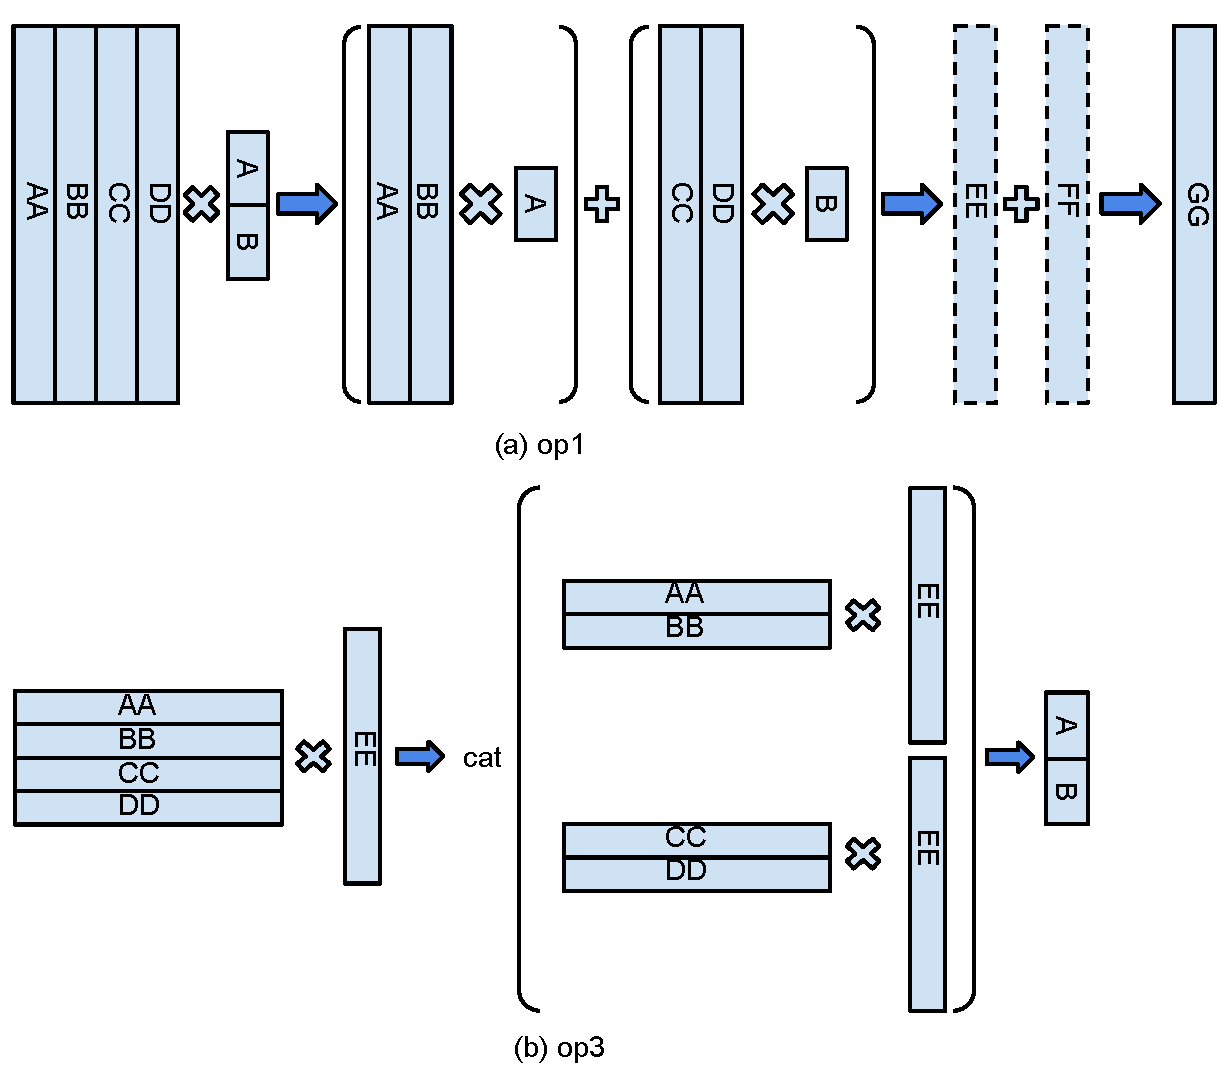
\includegraphics[scale=0.4]{./mat_group.pdf}
\vspace{-5pt}
\caption{Break a large group of dense matrices in an operation into multiple
small groups to reduce memory consumption. XX indicates a tall-and-skinny matrix
stored on SSDs and X indicates a small matrix stored in memory.}
\vspace{-5pt}
\label{fig:mat_group}
\end{figure}

The Anasazi eigensolvers frequently perform a matrix operation on many
tall-and-skinny matrices and the number of the matrices varies in each iteration.
The number of matrices can be as large as multiple hundred when an eigensolver
computes hundreds of eigenvalues.
Such an operation includes $op1$ and $op3$. If a thread has to read the data
in a row interval from all of the matrices, the amount of data in memory
can be very large and reading part of a partition results in many small reads
and writes to SSDs because the matrices are organized in column-major order.

Instead, we break a large group of tall-and-skinny matrices into multiple small
groups to reduce
memory consumption when evaluating these operations on them. Figure
\ref{fig:mat_group} illustrates this optimization on $op1$ and $op3$. For $op1$,
we split the small dense matrix horizontally and each group of tall-and-skinny
matrices gets a partition of the small dense matrix. Each group generates
a intermediate tall-and-skinny matrix conceptually and we apply an addition
operation on all intermediate matrices to generate the final result.
Materializing these
intermediate matrices would result in large memory consumption if we store them
in memory or large amount of I/O if we store them on SSDs. Instead, we leverage
the lazy evaluation in Section \ref{sec:lazy_eval}, i.e., we only materialize
part of them at a time and pass the materialized part to the addition operation
to generate the final result.

For $op3$, an eigensolver usually transopses a group of tall-and-skinny matrices
and multiply them with a tall-and-skinny matrix. We apply a similar strategy to
$op3$. We break the large group of dense matrices into multiple groups and each
group shares the same tall-and-skinny matrix on the right. Each group generates
a small matrix that can be kept in memory. In this case, all input matrices
are large and are stored on SSDs. To minimize I/O, we perform operations on
each group together to share I/O for accessing the tall-and-skinny matrix
on the right.

%\dz{This approach actually can change the computation complexity of dense matrix
%multiplication. I need to measure its impact on in-memory dense matrix
%multiplication.}

\subsubsection{Lazy evaluation} \label{sec:lazy_eval}
Lazy evaluation avoids materializing every dense matrix to reduce the amount
of data read and written to SSDs.
To enable lazy evaluation, we define a special matrix to represent the output
of a matrix operation. Such a matrix does not store the data of
an operation result. Instead, it stores the computation and a reference to
the input matrices. We refer to these special matrices as \textit{virtual matrices}.
Most matrix operations in Table \ref{anasazi_ops} output \textit{virtual matrices},
as long as the output matrices are tall-and-skinny matrices. Only \textit{op3}
and \textit{op6} cannot be evaluated lazily because they output small matrices
and small vectors and the output of these two operations is stored in Anasazi's
native matrices and vectors.

%With \textit{virtual matrices}, we construct a directed acyclic graph (DAG)
%at runtime to represent computation in FlashEigen. In the DAG, we store
%all scalar variables and small matrices as part of computation.
%Figure \ref{comp_seq} shows an example of a sequence of dense matrix operations
%performed in FlashEigen. Figure
%\ref{dag} visualizes the sequence of computation, which forms a directed acyclic
%graph (DAG). Inside this DAG, we do not need to perform any computation other
%than the last one.

All matrices in FlashEigen are immutable so that \textit{virtual matrices}
can generate the same result every time when they are materialized. Therefore,
our implementation of the matrix operations always generates new matrices.
The original Anasazi eigensolvers require in-place update on the existing dense
matrices, so FlashEigen only passes a pointer to a dense matrix to the Anasazi
eigensolvers instead of the matrix data. This approach is equivalent to variable
renaming used by compilers.
A dense matrix is garbage collected only when there are not any references to
the matrix.

%\textit{op7} and \textit{op8} access individual columns and have to be incorporated
%with the lazy evaluation. The eigensolvers usually access only one column at a time
%from a dense matrix. When accessing a single column, we materialize the virtual
%matrix in column major if the underlying matrix is a \textit{virtual matrix}.
%Because all matrices are immutable, setting a column in a matrix needs to
%copy the original matrix and set the particular column. Instead of physically
%generating the matrix, we create a virtual matrix that merge the original matrix
%with the column.

%\begin{figure}
%\begin{minted}[mathescape,
%		fontsize=\scriptsize,
%		frame=single,
%]{r}
%# MV0, MV1, MV2, MV3, MV4 are tall dense matrices.
%# B1, B2, B3, B4 are small dense matrices.
%# MV1 is the result of sparse matrix dense matrix
%# multiplication.
%MV0 <- rand_init
%MV1 <- SpMM
%MV2 <- 1 * MV0 * B1 + 0 * MV2
%MV2 <- 1 * MV2 * B2 + 0 * MV2
%MV3 <- 1 * MV1 * B3 + 0 * MV1
%MV1 <- -1 * MV2 * B4 + MV3
%MV4 <- MV1 * diag(vec)
%B <- t(MV4) * MV4
%\end{minted}
%\vspace{-5pt}
%\caption{A small sequence of dense matrix operations typically performed by
%the Anasazi eigensolvers.}
%\label{comp_seq}
%\end{figure}

%\begin{figure}
%\centering
%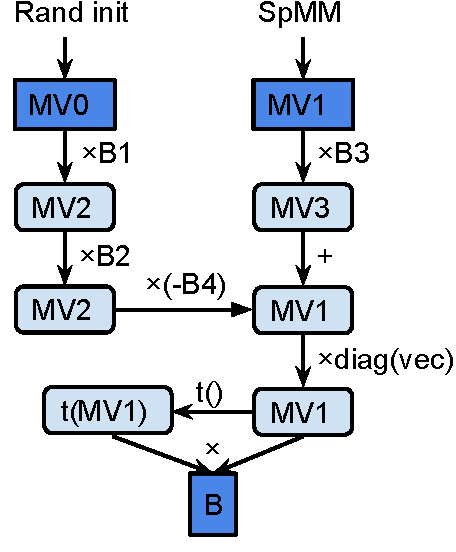
\includegraphics[scale=0.5]{./dag.pdf}
%\vspace{-5pt}
%\caption{A directed acyclic graph represents the sequence of matrix operations
%shown in Figure \ref{comp_seq}. Each rounded rectangular node indicates
%a virtual matrix and each rectangular node indicates a materialized matrix.}
%\vspace{-5pt}
%\label{dag}
%\end{figure}

To perform actual computation, FlashEigen needs to materialize
\textit{virtual matrices} in the two cases. FlashEigen materializes
a \textit{virtual matrix} when encountering \textit{op3} and \textit{op6}
because these two operations output Anasazi's native matrices and vectors.
Each \textit{virtual matrix} represent some computation on some materialized
tall-and-skinny matrices that are stored on SSDs. FlashEigen materializes
a \textit{virtual matrix}, which has more than one materialized input matrix,
to minimize the amount of data read from SSDs.
%FlashEigen also materializes all of the dense matrices in the basis.

A \textit{virtual matrix} may contain a sequence of operations, so materializing
it may trigger matrix materialization recursively.
We discard the materialized partition of a matrix, once it is no longer needed,
to avoid writing data of a intermediate \textit{virtual matrix} to SSDs.
We partition a \textit{virtual matrix} horizontally in the same fashion as
the external-memory matrices and materialize each partation independantly. 
To increase CPU cache hits, we use a much smaller partition size than
the external-memory matrix. As such, the output of the previous operation is
still in the CPU cache when it is fed to the next operation.

\subsubsection{Data and computation sharing in the DAG}
When materializing matrices in the DAG, we materialize them recursively.
As a result, the matrices that are depended by multiple other virtual matrices
potentially have to be materialized multiple times. Thus, we buffer the
recently materialized partitions temporarily to save I/O and computation.
We buffer the materialized partitions in the local thread, so accessing them
doesn't incur any locking overhead.
This is feasible because all tall matrices are partitioned horizontally and .

\dz{Only buffer data in the matrix where data can be shared.}

When we buffer the recent portions, we need to give each matrix a data identifier
to identify its data, so we can recognize which portion of data can be reused.
For certain operations, even though a new matrix is created, the data inside
remains the same. A typical example is transpose. The identifier we give to
each matrix should identify the data inside a matrix instead of individual matrices,
so a transposed matrix and its original matrix should share the same identifier.

We only cache one portion of data from each matrix. This is enough for the current
computation model.

The entire portion in the EM matrix should be processed by a single thread in order
to have the cached data being reused.

\subsubsection{Caching}

We can cache the most recently materialized matrix in memory.
